\documentclass[12pt,a4paper,faculty=ea,language=en,doctype=report]{ugent-doc}
\geometry{bottom=2.5cm,top=2.5cm,left=3cm,right=2cm} 
\renewcommand{\baselinestretch}{1.15}

\usepackage{fontspec}
\setmainfont{SourceSerifPro-Light.ttf}
\setsansfont{WorkSans-Regular.ttf}
\usepackage[english]{babel}
% \usepackage{libertine}
% \usepackage{libertinust1math}
\usepackage{amsmath} % math equations

% code snippets
\setmonofont{SourceCodePro-Regular.ttf}
\usepackage{listings}

% transcriptions:
\usepackage{xparse}
\usepackage{enumitem}

% acronyms
\usepackage[printonlyused,withpage]{acronym}

% figures
\usepackage{graphicx} 
\graphicspath{{./figures/}}

% Bibliography
\usepackage[backend=biber, style=apa, sorting=nyt, hyperref=true]{biblatex} 
\addbibresource{references.bib}
\usepackage{csquotes} % Suggested when using babel+biblatex

% Ugent specific
\usepackage[colorlinks=true, allcolors=ugentblue]{hyperref} % Hyperreferences
\usepackage[parfill]{parskip} % Whitespace between paragraphs and no indentation
\definecolor{mygreen}{rgb}{0,0.6,0}
\definecolor{mygray}{rgb}{0.5,0.5,0.5}
\definecolor{mymauve}{rgb}{0.58,0,0.82}
\definecolor{mygray}{rgb}{0.95, 0.95, 0.95}
\lstset{ %
  backgroundcolor=\color{mygray},  % choose the background color
  breaklines=true,                 % automatic line breaking only at whitespace
  captionpos=b,                    % sets the caption-position to bottom
  commentstyle=\color{mygreen},    % comment style
  escapeinside={\%*}{*)},          % if you want to add LaTeX within your code
  keywordstyle=\color{blue},       % keyword style
  stringstyle=\color{mymauve},
  basicstyle=\footnotesize\ttfamily
}

% styling table of contents
% \setcounter{tocdepth}{4}
% \setcounter{secnumdepth}{4}


% ---------------------------------------------

\thesubtitle{Linked Data}
\usepackage{ulem} % for colored underline
\renewcommand{\ULthickness}{2pt} % adjust thickness of underline
\thetitle{\uline{\color{ugentblue} Augmented Reality visualisation on site: \\ BIM semantics and communication}}
\infoboxa{\bfseries\large Master's dissertation submitted in order to obtain the academic degree of \\
Master of Science in de ingenieurswetenschappen: architectuur
}
\infoboxb{Supervisor: 
\begin{tabular}[t]{lll}
    Prof.\ ir.-arch.\ Paulus Present\\ % note syntax 'short space'
\end{tabular}
}
\infoboxc{Counselors: 
\begin{tabular}[t]{lll}
    Ir.-arch.\ Jeroen Werbrouck\\ % note syntax 'short space'
    Prof.\ dr.\ ir.\ arch.\ Ruben Verstraeten
\end{tabular}
}

\infoboxd{Philippe Soubrier 01702837 philippe.soubrier@ugent.be}
\infoboxe{Academic year: 2022--2023}

% ---------------------------------------------
\begin{document}
\maketitle
\renewcommand{\ULthickness}{1pt}
{\hypersetup{hidelinks}\tableofcontents} % hide link color in toc
\listoffigures
\newpage

\chapter*{Short abstract}
This is my short abstract.
\chapter*{Abstract}
This is my abstract
\chapter{Introduction}
\section{Context}
\subsection{3D viewers}
-> Applications?

-> Who uses them?

-> What for?

\subsection{\acs{bim} geometry} \label{subsec:bimGeometry}
% -> What is \ac{bim}? (short)

% -> Extend of \ac{bim} geometry?
% -> Complexity of \ac{bim} geometry?
The 3D model of a building consists of a multitude of sub-models, describing objects for all the different stakeholders participating to the porject. Some describe very large objects, and some very small parts. Both can be defined in there most simple and abstract form or have an intricate and complex geometry. As a basic example, can a door simply be defined as a box, or up to the level of the screw-thread for the hinge system. The level of abstraction is here described as the \ac{lod} and is most of the time pre-selected for the needs of a \ac{bim} model, and is applied throughout a single model.

\begin{figure}
    \centering
    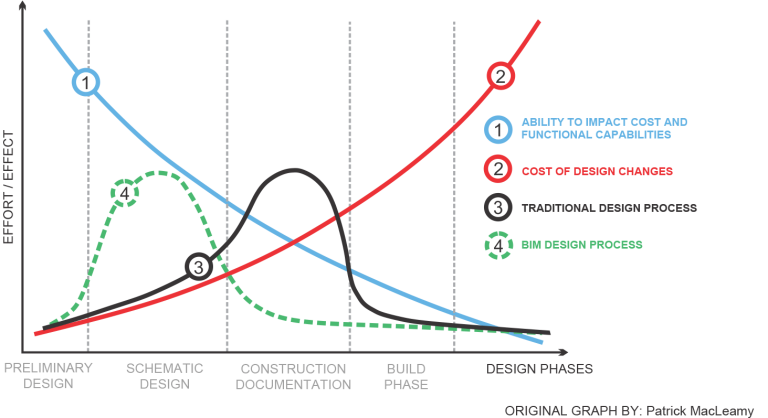
\includegraphics[width=0.5\textwidth]{figures/BIM grafiek.png}
    \caption{Evolution of \ac{lod} during the life-cycle of a building.}
    \label{fig:bimGraph}
\end{figure}

As shown in figure~\ref{fig:bimGraph}, a standard BIM workflow goes through multiple fases each with there assosiated model and \ac{lod}. The \ac{lod} is a very important concept in the \ac{aec} industry, as it allows for a very efficient workflow. Approaching the modeling step from a top-down perspective, starting with rougher geometries descriving the rougher ideas of a concept model and evoluting to a more refined model for the construction fase. As last and longest standing model, can a higher \ac{lod} be used to describe suttle changes in the evolution of a building.

This amount of data, both accounting for the \\
-> Some data BB models

\subsection{\acs{ldbim}}
% -> ! Focus on geometry

% -> What is \ac{ldbim}?

% -> Why the need / What are the advantages of \ac{ldbim}?

% -> Context od enrichment and complexity

-> Own definition of \ac{ldbim}

The interconnectivity of semantics can also be applied to geometry descriptions. Which could allow the co-existance of multiple \ac{lod}'s in a single model. Besides storing the evolution of an single element's geometry, it allows the linking of the different \ac{lod}'s to each other. In contrary to a standard \ac{bim} models, as explained in \ref{subsec:bimGeometry}.

\subsection{Computing power dilemma}
The enrichment of the \ac{ldbim}-graph also comes with a cost. The amount of data that needs to be stored and processed is much larger than a standard \ac{bim} model. Viewers greatly suffer from enrichment as most standard applications require the full model to be loaded in memory.

-> What is the hardware problem?

-> Why is it that important for the \ac{aec} industry?

\section{Research questions}

-> Why the need for this thesis? (why a \ac{ldbim} viewer?)

-> What is the possible solution? (Culling algorithms)

-> Why the need for research questions?
(culling algorithms are not new, always progress, see later)

\subsection[Can \acs{ldbim} be culled?]{To which extent can \acs{ldbim} geometry be culled\\
    to be streamed to lightweight viewers?}
-> What can be culled exactly?

-> What needs to be streamed?

-> What is the impact of culling on the viewing experience?

\subsection[Can existing semantic be used?]{Can existing semantic and ontologies be used to\\
    feed possible culling algorithms?}
-> What are ontologies?

-> Can GIS ontologies be used too?

-> What are the advantages of using ontologies?

\section{Research objectives}
\subsection[Advantages of LDBIM]{Bring forward the advantages of \acs{ldbim} for visualization of big 3D models}
-> Showcase that existing models are already mature enough for these usecases.

->
\subsection[Showcase the fisability]{Showcase the fisability of \acs{ldbim} for visualization of big 3D models}
->
\setlist[description]{
  font={\sffamily\bfseries},
  labelsep=0pt,
  labelwidth=\transcriptlen,
  leftmargin=\transcriptlen,
}

\newlength{\transcriptlen}

\NewDocumentCommand {\setspeaker} { mo } {%
  \IfNoValueTF{#2}
  {\expandafter\newcommand\csname#1\endcsname{\item[#1:]}}%
  {\expandafter\newcommand\csname#1\endcsname{\item[#2:]}}%
  \IfNoValueTF{#2}
  {\settowidth{\transcriptlen}{#1}}%
  {\settowidth{\transcriptlen}{#2}}%
}

% Easiest to put the longest name last...
\setspeaker{me}[Me]
\setspeaker{gpt}[GPT chat]

% How much of a gap between speakers and text?
\addtolength{\transcriptlen}{1em}%

\chapter*{GPT chat}
\scene[]
\StageDir{
    \begin{center} Table of contents
     \end{center}
}
\begin{drama}
\mespeaks What is linked data?
\gptspeaks Linked data is a way of representing and sharing data on the internet so that it can be easily linked to related data and more easily used by machines. This is achieved by using standardized formats and protocols, such as RDF (Resource Description Framework), which allows data from different sources to be connected and used together. The goal of linked data is to create a web of interconnected data that can be easily accessed and used by anyone, with the ultimate aim of enabling people and machines to better understand the world around them.
\mespeaks What are the opportunities for the AEC industry?
The AEC (architecture, engineering, and construction) industry has many opportunities to benefit from linked data. For example, linked data can be used to more easily share and integrate data from different sources, such as building information models (BIM) and GIS (geographic information systems), which can help improve collaboration and decision-making among different stakeholders in a construction project. Linked data can also be used to create more accurate and detailed models of buildings and infrastructure, which can help improve the design and planning of projects. Additionally, linked data can be used to create more comprehensive and accessible datasets that can be used for research and analysis, helping to drive innovation and progress in the AEC industry.
\mespeaks Will the ifc format still have a future?

\end{drama}
\clearpage
\section*{URIs}
\begin{description}
	\me What are URI

	\gpt A URI, or Uniform Resource Identifier, is a string of characters that identify a name or a resource on the Internet. URIs can be broken down into two types: URLs and URNs. A URL, or Uniform Resource Locator, is the web address of a specific page or file on the internet, while a URN, or Uniform Resource Name, is a unique identifier for a resource that may or may not be available on the internet. For example, "http://www.example.com" is a URL, while "urn:isbn:978-1-60309-024-3" is a URN

	\me does everything have a uri in an rdf graph?

	\gpt In an RDF graph, every resource is identified by a URI. The URI serves as a unique identifier for the resource, and it can be used to refer to the resource in RDF statements. The URI can be thought of as the name of the resource, and it is used to distinguish the resource from other resources in the graph.

	\me but does every triple have a uri?

	\gpt In an RDF graph, every resource is identified by a URI, but not every triple necessarily has a URI. A triple in an RDF graph consists of a subject, a predicate, and an object, and each of these components can be either a URI or a literal value. In some cases, all three components of a triple may be URIs, while in other cases, one or more of the components may be a literal value. For example, the following triple has a URI for the subject and predicate, but the object is a literal string:

	\begin{lstlisting}[language=SPARQL]
`<http://www.example.com/books/book1> <http://www.example.com/ns/title> "The Great Gatsby"`	
\end{lstlisting}

	In this triple, the subject is the URI http://www.example.com/books/book1, the predicate is the URI http://www.example.com/ns/title, and the object is the string "The Great Gatsby".

	\me why does querying ressources gives back uri's?

	\gpt When you query a resource in an RDF graph, the response typically includes the URI of the resource. The URI serves as a unique identifier for the resource, and it can be used to refer to the resource in other queries or statements. Additionally, the URI may be used to dereference the resource and retrieve additional information about it.

	\me Is that ressource URI automatically assigned by the sparql endpoint you are querying?

	\gpt The URI for a resource in an RDF graph is not automatically assigned by a SPARQL endpoint. In most cases, the URI for a resource is determined by the creator of the RDF data, and it is typically chosen to be a unique and meaningful identifier for the resource. For example, a URI for a book might include the title of the book and the author's name, while a URI for a person might include their full name and date of birth. The URI is then used to identify the resource in the RDF data, and it can be used to query the resource using a SPARQL endpoint.

	\me can you give me an example of triple data with an ressource uri?

	\gpt Sure, here is an example of a triple with a resource URI:

	\begin{lstlisting}[language=SPARQL]
`<http://www.example.com/books/book1> <http://www.example.com/ns/title> <http://www.example.com/ns/TheGreatGatsby>`	
\end{lstlisting}

	In this triple, the subject is the URI http://www.example.com/books/book1, the predicate is the URI http://www.example.com/ns/title, and the object is the URI http://www.example.com/ns/TheGreatGatsby.
	The subject of this triple identifies a specific book, the predicate specifies that the object of the triple is the title of the book, and the object is the URI of the resource that represents the title of the book. This URI could be used in other triples to provide additional information about the title of the book, such as the language in which it was written or the author who wrote it.

	\me Does that uri then directly refers to data? I mean, can I look it up in my browser, or is it just semantics for the sparql endpoint?

	\gpt A URI in an RDF graph typically does not directly refer to data that can be looked up in a web browser. Instead, the URI serves as a unique identifier for a resource in the RDF graph, and it is used to distinguish that resource from other resources in the graph. The URI itself does not contain any information about the resource, but it can be used to retrieve additional information about the resource through a process called dereferencing.
	To dereference a URI, you can send a request to the URI using a web client, such as a web browser or a SPARQL endpoint. If the URI is associated with a resource that is available on the internet, the request will return information about the resource. For example, if the URI identifies a web page, the request will return the contents of the web page.
	However, not all URIs are associated with resources that are available on the internet. In some cases, the URI may simply serve as a unique identifier for a concept or an idea, without referring to any specific data. In these cases, dereferencing the URI will not return any information about the resource.

	\dots
\end{description}
\clearpage
\section*{RDF reasoners}
\begin{description}
	\me What is a rdf reasoner?
	
	\gpt An RDF reasoner is a type of software that can automatically infer new information based on existing data in an RDF (Resource Description Framework) graph. An RDF graph is a way of representing information using the RDF data model, which is a set of interconnected statements about resources. For example, if an RDF graph contains statements that indicate that a particular person is the child of a certain parent, an RDF reasoner could infer that the person is also the sibling of the parent's other children. In this way, an RDF reasoner can help to automatically organize and make sense of complex data in an RDF graph.
	
	\me Does it add data to the graph or is only used for the query?
	
	\gpt An RDF reasoner does not add data to the RDF graph directly. Instead, it analyzes the existing data in the graph and uses rules of inference to automatically generate new statements that can be added to the graph. These new statements are typically derived from the existing data in the graph and reflect relationships or connections that can be logically inferred from that data. For example, if an RDF graph contains statements indicating that person A is the child of person B, and person B is the child of person C, an RDF reasoner could infer that person A is the grandchild of person C and generate a new statement to that effect. In this way, an RDF reasoner can help to enrich the data in an RDF graph and make it more useful for querying and analysis.
	
	\me Does it then run continuously, searching for new correlations?
	
	\gpt It depends on the specific implementation of the RDF reasoner. Some RDF reasoners may be designed to run continuously, continuously analyzing the data in an RDF graph and generating new statements as needed. Other RDF reasoners may be designed to run only when explicitly invoked by a user or application, in which case they would not be continuously searching for new correlations. In general, whether an RDF reasoner runs continuously or not will depend on the specific requirements and goals of the system in which it is being used.
	
	\me Is it part of the triplestore or the sparql endpoint?
	
	\gpt An RDF reasoner is not necessarily part of a triplestore or a SPARQL endpoint. A triplestore is a type of database specifically designed for storing and managing RDF data, while a SPARQL endpoint is a web service that allows users to query an RDF graph using the SPARQL query language. An RDF reasoner, on the other hand, is a type of software that can automatically infer new information from an RDF graph, but it is not necessarily part of a triplestore or a SPARQL endpoint. In some cases, an RDF reasoner may be used in conjunction with a triplestore or a SPARQL endpoint as part of a larger system for managing and querying RDF data. In other cases, an RDF reasoner may be used independently of these technologies.
	
	\me Wait a minute. Does all triplestores have sparql endpoints?
	
	\gpt Not all triplestores have SPARQL endpoints. A triplestore is a type of database specifically designed for storing and managing RDF data, while a SPARQL endpoint is a web service that allows users to query an RDF graph using the SPARQL query language. A triplestore and a SPARQL endpoint are separate, but related, technologies. A triplestore provides a backend storage mechanism for RDF data, while a SPARQL endpoint provides a way for users to access and query that data. In some cases, a triplestore may include a SPARQL endpoint as part of its functionality, allowing users to query the data stored in the triplestore using SPARQL. In other cases, a triplestore may not include a SPARQL endpoint, and a separate SPARQL endpoint may need to be used in order to query the data stored in the triplestore.
	
	\me how would a sparql endpoint talk to a separate triplestore? By using lots of http requests?
	
	\gpt A SPARQL endpoint can talk to a separate triplestore by using a network protocol such as HTTP to send SPARQL queries to the triplestore and receive the results of those queries. The exact details of how this communication occurs will depend on the specific implementation of the SPARQL endpoint and the triplestore. In some cases, the SPARQL endpoint and the triplestore may be part of the same system and may be designed to communicate with each other using a custom, proprietary protocol. In other cases, the SPARQL endpoint and the triplestore may be part of separate systems and may communicate with each other using a standard network protocol such as HTTP. In either case, the goal is to allow the SPARQL endpoint to send queries to the triplestore and receive the results of those queries in a way that is efficient and transparent to the user.
	
	\me So a triplestore CAN interpret sparql queries?
	
	\gpt A SPARQL endpoint is a web service that allows users to query an RDF graph using the SPARQL query language. It provides a convenient way for users to access and query RDF data without having to directly interact with the underlying triplestore. This can be useful in a number of situations. For example, a SPARQL endpoint can provide a standard, consistent interface for querying RDF data, allowing different applications and users to access the data in the same way. Additionally, a SPARQL endpoint can provide additional features and functionality beyond what is available in a triplestore, such as support for querying multiple RDF graphs, advanced query optimization, and caching of query results. In this way, a SPARQL endpoint can provide a useful layer of abstraction between the triplestore and the applications and users that need to access the data stored in the triplestore.
	
	\me So, in a certain way it is a standardisation of the querying?
	
	\gpt Yes, you could say that a SPARQL endpoint provides a standardized interface for querying RDF data. The SPARQL query language is a standardized, widely-used language for querying RDF data, and a SPARQL endpoint provides a way for users and applications to access RDF data using this standard language. This can help to ensure that different applications and users are able to access RDF data in a consistent and predictable way, regardless of the specific triplestore or other backend technology being used to store the data. In this way, a SPARQL endpoint can help to promote interoperability and facilitate the use of RDF data in a variety of different contexts.

	\dots
\end{description}
\clearpage
\section*{Linked Data and \ac{bim}}
\begin{description}
	\me What are the disadvantages of linked data for the AEC industry? Specifically when it comes to communication on the building site?

	\gpt
	\begin{enumerate}
		\item The complexity of linked data can be overwhelming and difficult to understand for those without a strong technical background. This can hinder communication on the building site and lead to misunderstandings or errors.
		\item Linked data often requires specialized software and tools to access and interpret, which may not be readily available on the building site. This can make it difficult for teams to share and collaborate on information in real-time.
		\item The sheer volume of data that is generated and linked through the use of linked data can be overwhelming, making it difficult to identify and access the specific information that is needed for a particular project or task.
		\item The integration of linked data into existing systems and processes can be time-consuming and costly, requiring significant training and resources to implement effectively.
		\item The security and privacy of linked data can be a concern, as the interconnected nature of the data means that any breach or unauthorized access could potentially affect multiple systems and parties.
	\end{enumerate}
	Overall, the disadvantages of linked data for the AEC industry include a potential lack of understanding and specialized tools, difficulty managing and accessing data, and concerns over security and privacy.


	\me Which type of software could help for that matter?
	\gpt
	\begin{enumerate}
		\item There are several types of software that could help with the challenges of linked data in the AEC industry, including:
		\item Collaboration and project management software, such as Asana or Trello, which can help teams to organize and share information in real-time.
		\item Data visualization and analysis tools, such as Tableau or Qlik, which can help to make sense of large volumes of linked data and identify patterns and trends.
		\item Data management and governance platforms, such as Talend or Informatica, which can help to ensure the integrity and security of linked data, as well as facilitate its integration into existing systems and processes.
		\item Linked data tools, such as Apache Jena or GraphDB, which can help to create, manage, and query linked data sets.
	\end{enumerate}
	Overall, the use of specialized software can help to overcome the challenges of linked data in the AEC industry, enabling teams to better communicate, collaborate, and make sense of the data.

	\me Which type of software could take advantage of linked data on the building site itself?

	\gpt There are several types of software that could take advantage of linked data on the building site itself, including:
	\begin{enumerate}
		\item Augmented reality (AR) and virtual reality (VR) tools, such as HoloLens or Sketchfab, which can enable teams to visualize and interact with linked data in real-time, providing a more immersive and intuitive way of understanding complex information.
		\item Sensors and IoT technologies, such as BIM sensors or connected devices, which can generate and link data in real-time from the building site, providing teams with real-time insights and updates on the status and performance of the project.
		\item Building information modeling (BIM) software, such as Autodesk Revit or ArchiCAD, which can help teams to create and manage linked data sets that represent the design, construction, and operation of a building, providing a comprehensive and integrated view of the project.
	\end{enumerate}
	Overall, the use of specialized software can help teams to take advantage of linked data on the building site itself, enabling them to better understand and manage the project in real-time.

	\me What would be the greatest challenge for AR on the construction site, using linked data?

	\gpt The greatest challenge for AR on the construction site, using linked data, would be ensuring that the data is accurate, up-to-date, and properly linked.
	As linked data is often generated from multiple sources and can be updated in real-time, it is critical that the data is accurate and consistent across all systems and stakeholders. This can be a challenge, as errors or inconsistencies in the data could lead to misunderstandings or errors on the construction site.
	Additionally, ensuring that the data is properly linked and interconnected can also be a challenge, as it requires specialized knowledge and tools to create and manage linked data sets. This can be a barrier for teams that are not familiar with linked data and its potential benefits.
	Overall, the greatest challenge for AR on the construction site, using linked data, would be ensuring the accuracy, consistency, and connectivity of the data, in order to support effective decision-making and collaboration on the building site.

\end{description}
\clearpage
\section*{\ac{chc}}
\begin{description}
	\me Can you explain me the Coherent Hierarchical Culling algorithm?

	\gpt Coherent Hierarchical Culling (CHC) is an algorithm used in computer graphics to improve the performance of rendering 3D scenes by reducing the number of objects that need to be processed by the graphics pipeline. The goal of CHC is to quickly and efficiently determine which objects in a scene are visible to the viewer and which objects are occluded (hidden) by other objects and therefore do not need to be drawn. This can greatly improve the performance of a graphics application, especially when dealing with complex or large scenes.

	CHC works by dividing the scene into a hierarchy of bounding volumes, with each level of the hierarchy representing a different level of detail. The hierarchy is constructed so that each bounding volume encloses one or more objects in the scene, and the bounding volumes at higher levels of the hierarchy enclose groups of objects at lower levels.

	The CHC algorithm begins by determining the bounding volume at the top level of the hierarchy that encloses the viewer's current viewpoint. It then uses this bounding volume to recursively traverse the hierarchy and identify the objects that are potentially visible to the viewer. As the algorithm traverses the hierarchy, it eliminates objects and bounding volumes that are completely occluded by other objects or bounding volumes. This process continues until the algorithm reaches the lowest level of the hierarchy, at which point it has a list of the objects that are potentially visible to the viewer.

	CHC is an efficient algorithm because it can quickly eliminate large groups of objects and bounding volumes that are not visible to the viewer, reducing the number of objects that need to be processed by the graphics pipeline. It is also a "coherent" algorithm because it takes advantage of spatial coherence in the scene, meaning that objects that are near each other in the scene are likely to be occluded by similar objects. This allows the algorithm to quickly eliminate large groups of objects that are occluded by other objects.

	\me How does it compute if a bounding volume is completely occluded?

	\gpt In the Coherent Hierarchical Culling (CHC) algorithm, the occlusion of a bounding volume is determined by comparing it to other bounding volumes in the scene. Specifically, the algorithm compares the bounding volume being tested to the bounding volumes of other objects in the scene to see if it is completely contained within another bounding volume. If the bounding volume being tested is completely contained within another bounding volume, it is considered to be occluded and is eliminated from further processing.

	To determine if one bounding volume is completely contained within another bounding volume, the CHC algorithm compares the vertices of the bounding volume being tested to the planes of the bounding volume it is being compared to. If all of the vertices of the bounding volume being tested lie on the same side of all of the planes of the other bounding volume, then the bounding volume being tested is completely contained within the other bounding volume and is considered occluded.

	There are several different types of bounding volumes that can be used with the CHC algorithm, including axis-aligned bounding boxes (AABBs), oriented bounding boxes (OBBs), and bounding spheres. The specific method for determining occlusion will depend on the type of bounding volume being used.

	\me Can you explain it all again in simpler terms? I am confused about what bounding volumes actually are.

	\gpt Certainly! Coherent Hierarchical Culling (CHC) is an algorithm used to improve the performance of rendering 3D graphics by reducing the number of objects that need to be processed. It does this by dividing the scene into a hierarchy of bounding volumes, with each level of the hierarchy representing a different level of detail.

	A bounding volume is a geometric shape that encloses an object or group of objects in the scene. The bounding volume is typically chosen to be as small as possible while still enclosing the object or objects it represents. There are several different types of bounding volumes that can be used, including axis-aligned bounding boxes (AABBs), oriented bounding boxes (OBBs), and bounding spheres.

	The CHC algorithm begins by determining the bounding volume at the top level of the hierarchy that encloses the viewer's current viewpoint. It then uses this bounding volume to recursively traverse the hierarchy and identify the objects that are potentially visible to the viewer. As the algorithm traverses the hierarchy, it eliminates objects and bounding volumes that are completely occluded by other objects or bounding volumes. This process continues until the algorithm reaches the lowest level of the hierarchy, at which point it has a list of the objects that are potentially visible to the viewer.

	To determine if a bounding volume is occluded, the CHC algorithm compares it to the bounding volumes of other objects in the scene. If the bounding volume being tested is completely contained within another bounding volume, it is considered to be occluded and is eliminated from further processing. This allows the CHC algorithm to quickly eliminate large groups of objects that are not visible to the viewer, improving the performance of the graphics application.

	\me And in very simple terms, how does it compute if bounding volumes are occluded?

	\gpt To determine if a bounding volume is occluded (hidden) by another bounding volume, the Coherent Hierarchical Culling (CHC) algorithm compares the vertices of the bounding volume being tested to the planes of the bounding volume it is being compared to. If all of the vertices of the bounding volume being tested lie on the same side of all of the planes of the other bounding volume, then the bounding volume being tested is considered to be completely contained within the other bounding volume and is therefore occluded.

	For example, if the bounding volume being tested is an axis-aligned bounding box (AABB) and the bounding volume it is being compared to is also an AABB, the CHC algorithm would compare the vertices of the AABB being tested to the planes of the other AABB. If all of the vertices of the AABB being tested lie on the same side of all of the planes of the other AABB, then the AABB being tested is considered to be occluded.

	This process is repeated for each bounding volume in the scene, allowing the CHC algorithm to quickly eliminate objects and bounding volumes that are not visible to the viewer and improve the performance of the graphics application.

	\me A bounding volume A sitting inside another bounding volume B means all of the geometry in A is not visible outside of B?

	\gpt Yes, that's correct! If a bounding volume (A) is completely contained within another bounding volume (B), it means that all of the geometry represented by bounding volume A is completely occluded (hidden) by the geometry represented by bounding volume B. This is because the geometry represented by bounding volume A is completely enclosed by the geometry represented by bounding volume B, and therefore none of it is visible to the viewer.

	In the context of the Coherent Hierarchical Culling (CHC) algorithm, this means that the objects represented by bounding volume A can be eliminated from further processing, since they are not visible to the viewer. This can greatly improve the performance of a graphics application, especially when dealing with complex or large scenes.

	\dots
\end{description}

  
\chapter{State of the art}
  \section{\acs{ar} on-site approaches}
    \subsection{Autodesk xyz - Atom}
    \subsection{Openspace AI}    

  \section{Linked geometric data}
    \subsection{\acs{bot}}
    \subsection{\acs{ifcowl}}
    \subsection{Other ontologies} 
      \subsubsection{\acs{bcfowl}}
  
  \section{\acs{ldbim} viewers}
    \subsection{ld-bim.web.app}

  \section{Rendering optimizations}
    \subsection{Culling algorithms}
      \subsubsection{Bounding Box Culling}
      \subsubsection{Frustum Culling}
      \subsubsection{Octree Culling}
      \subsubsection{Quadtree Culling}
      \subsubsection{Spatial Hashing}
      \subsubsection{Spatial Partitioning}
      \subsubsection{Visibility Culling}
      \subsubsection{Z-Buffer Culling}
      \subsubsection{Coherent Hierarchical Culling}
    \subsection{Qonic}

\chapter{Methodology}
  \section{\acs{rdf} data}
    \subsection{Existing data}
    \subsection{Adding data}
  \section{\acs{lod} streaming model}  
    \subsection{Culling}
    \subsection{Redundancy avoidance with \acs{bcf} history}
  \section{Querying}
    \subsection{Front-end}
    \subsection{Back-end}
  \section{Rendering}
    \subsection{Three.js}
    \subsection{Shaders}

\chapter{Website}
  \section{Setup}
    \subsection{Software}
    \subsection{Hardware}
  \section{User interface}

\chapter{Results}


% \appendix
% \chapter{First appendix}
this is my first appendix
\clearpage
\chapter*{List of Acronyms}
\begin{acronym}[JSONP]\itemsep2pt\hypersetup{hidelinks}
  \acro{ar}[AR]{Augmented Reality}
  \acro{aec}[AEC]{Architecture, Engineering and Construction}
  \acro{bcf}[BCF]{\acs{bim} Collaboration Format}
  \acro{bcfowl}[bcfOWL]{\acs{bim} Collaboration Format Ontology}
  \acro{bim}[BIM]{Building Information Modeling}
  \acro{bot}[BOT]{Building Topology Ontology}
  \acro{chc}[CHC]{Coherent Hierarchical Culling algorithm}
  \acro{gltf}[GLTF]{GL Transmission Format}
  \acro{hhd}[HHD]{Hand Held Device}
  \acro{ifc}[IFC]{Industry Foundation Classes}
  \acro{ifcowl}[ifcOWL]{Industry Foundation Classes Ontology}
  \acro{ldbim}[LDBIM]{Linked Data \acs{bim}}
  \acro{lod}[LOD]{Level of Detail}
  \acro{owl}[OWL]{Web Ontology Language}
  \acro{rdf}[RDF]{Resource Description Framework}
  \acro{rdfs}[RDFS]{Resource Description Framework Schema}
  \acro{sparql}[SPARQL]{SPARQL Protocol and RDF Query Language}
\end{acronym}

\printbibliography[heading=bibintoc,title={References}]
\end{document}
